\chapter{Concepts}

This chapter is split into three parts. Each part discusses a basic concept of Computer Science and its corresponding exercises.

\section{Representing Information with Symbols}
\label{section:representing_information_with_symbols}

Representing information with symbols is a fundamental concept of Computer Science as information should be represented clear and concisely. Words can be seen as a sequence of symbols, namely a sequence of letters.

\subsection{Similar Words}

Transmitting information includes representing it in a message, sending it to the destination and the receiver being able to make sense of it even tough the message might contain errors such as a spelling mistake. To achieve this sender and receiver agree to only send messages with a minimal editing distance \cite{AnD} between each of them. 

\subsection*{Editing distance}

The editing distance is the amount of operations that need to be done to transform a message in another. Operations are deleting, inserting and changing a letter \TODO{add some TI explanation}. A cost function exists that defines the cost of each operation, and in our case each operation has a cost of 1 (unit cost model). The editing distance is then the minimal cost to transform a message into another one by a sequence of operations. In our case a message is a word.

\begin{example}
    The editing distance between \code{LIKE} and \code{BIKE} is 1, since changing the first letter from an \code{L} to and \code{B} transforms the first word into the second.
\end{example}

If sender and receiver agree to only transmit words with a minimal editing distance of e.g 3, then the receiver can still uniquely determine what word the sender has sent even when at most 1 spelling mistake has been made. The receiver calculates the minimal editing distance between the received word and each of the agreed words and chooses the word with the least editing distance.
The receiver assume that this was the word the sender wanted to sent. This of course work only if there are not more than 1 error in the word. If this happens the editing distance to another word is closer than to the original word and hence the word is misinterpreted. To counter this, sender and receiver might agree on a bigger minimal distance, but this comes with a tradeoff. When chosing a bigger minimal distance for a fixed alphabet, the number of words that can be used shrinks. To maintain the same amount of words the size of the lphabet can be increased too, resulting in longer words.

The purpose of the \code{similar words} exercises is to learn these operations. Therefore an exercise is dedicated to each opertion: adding, changing and removing a letter from a word. Additionally, an exercise about swapping adjacent letters in a word is included. Swapping adjacent letters is not part of the mentioned operations and usually consists of 2 operations: removing and adding or changing twice. However, when typing on a keyboard typing mistakes happen often and most of the time only two adjacent letters are swapped. This exercises is supposed to train the ability to spot these sort of mistakes.

\subsection*{Adding a letter}

In the \code{adding a letter} exercise pupils are presented a word, the alphabet from A to Z and spaces between each letter of the word as well as at the beginnig and the end of the word, where a letter can be added. Pupils are supposed to choose a letter from the alphabet and add it to one of the mentioned spaces to form a new valid word.

\begin{example}
    The word \code{PACE} is given. By adding the letter \code{S} before the first letter, the valid word \code{SPACE} is formed.
\end{example}

\subsection*{Changing a letter}

In this exercise there is again a word and the alphabet from A to Z shown. Again pupils should select a letter from the alphabet, but this time, instead of adding it to a space, the selected letter should be replace a letter from the word itself to create a new valid word.

\begin{example}
    The word \code{BIKE} is given. By changing the first letter from a \code{B} to a \code{L} the new valid word \code{LIKE} is formed.
\end{example}

\subsection*{Removing a letter}

In this exercise pupils receive a word and they should select a character from within the word an move it to the trashcan to remove the letter from the word itself to form a new valid word.

\begin{example}
    The word \code{SPACE} is given. By removing the first letter the new valid word \code{PACE} is formed.
\end{example}

\subsection*{Swapping two adjacent letters}

To learn to recognize typing mistakes in a word pupils are presented a word with swapped adjacent letters and they are supposed to identify those and swap them back to restore to original word. Here are multiple difficulty levels possible, where on the easy level only one pair of adjacent letters is swapped and on harder levels multiple pairs of adjacent letters are swapped.

\begin{example}
    The word \code{BKIE} is given. By swapping the second and third letter the original word \code{BIKE} is restored.
\end{example}

\subsection{Representing Numbers like the Maya}

Today one is used to the decimal number system (base number 10), with 10 symbols. The Maya used a different number system with with a base number of 20 i.e the vigesimal number system. It is believed that the Maya used their ten fingers and ten toes to count adding up to twenty. But instead of having a symbol for each number as in the decimal system, the Maya used three different symbols: zero (a turtle shell, belly side up), one (a dot) and five (a bar) \cite{Maya}. The mayan representation of the decimal number from 0 to 19 can be found in figure \ref{fig:maya_numerals}.

\begin{figure} 
    \centering
    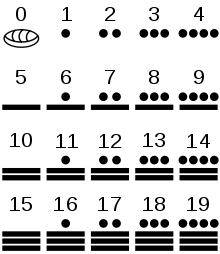
\includegraphics[width=0.3 \columnwidth]{figures/maya_number_system.png}
    \caption{Representation of the Maya numbers from 0 to 19} 
    \label{fig:maya_numerals} 
\end{figure}

The following exercises are supposed to familiarize pupils with a new number system, the mayan number system. First converting numbers between the decimal number system and the mayan numbers is trained topped of an exercise about adding two mayan numbers.

\subsection*{Representing mayan numbers}

A decimal number is presented to the pupils and they need to choose the correct amount of dots and bars representing the decimal number. For the purpose of simplicity, only decimal numbers between 1 and 19 are chosen.

\begin{example}
    The decimal number \code{17} is writte as three bars and two dots.
\end{example}

\subsection*{Understanding mayan numbers}

In this exercise the pupils learn to understand mayan numbers. Again only decimal numbers between 1 and 19 are used and the pupils need to understand what mayan number is shown and write down the decimal equivalent.

\subsection*{Adding mayan numbers}

To sum this section up, adding mayan numbers is learned. This exercises combines the previous two, since the pupils need to understand the summands given in the mayan number system, add them and write the sum down in either decimal number system or the mayan number system.

\subsection{Representing Numbers with Coins}

The following exercises introduce a new number system and trains an already learned one: the binary number system and the decimal number system. Both number systems are praticed with coins with numbers. The binary coins include the following numbers: 1, 2, 4, 8, 16, 32 and 64 (Fig. \ref{fig:binary_coins}). The decimal coins include 1, 2, 5, 10, 20 and 50 (Fig. \ref{fig:decimal_coins}). 
Overall, the same concepts are praticed for both number systems with the limitation that every binary coin can at most be used once. For both number systems the following exercises are given:
\begin{itemize}
    \item Conversion of a decimal number to its coin representation
    \item Conversion of a number given in its coin representation to a decimal number
\end{itemize}
Additionally, for the decimal number system the following exercise is given:
\begin{itemize}
    \item Reducing the number of decimal coins in a given set of decimal coins
\end{itemize}

\begin{figure} 
    \centering
    
\includegraphics[width=0.5 \columnwidth]{figures/decimal_coins.png}
    \caption{Representation of the decimal coins} 
    \label{fig:decimal_coins} 
\end{figure}

\begin{figure} 
    \centering
    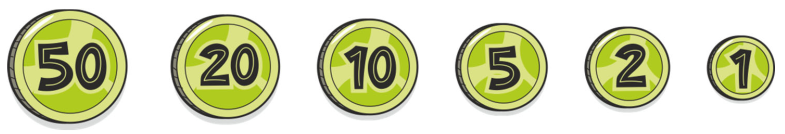
\includegraphics[width=0.5 \columnwidth]{figures/binary_coins.png}
    \caption{Representation of the binary coins} 
    \label{fig:binary_coins} 
\end{figure}

\subsection*{Conversion of a decimal number to its coin representation}

This exercise includes two difficulty levels:
\begin{itemize}
    \item Converting a decimal number to a coin representation, where the sum of all coins are equal to the decimal number
    \item Converting a decimal number to a coin representation, where the sum of all coins are equal to the decimal number \textbf{and} the amount of used coins is minimal.
\end{itemize}

\subsection*{Conversion of a number given in its coin representation to a decimal number}

This exercise is straigh forward. A number given in its coin representation, either binary or decimal coins, have to be converted to a decimal number. 

\subsection*{Reducing the amount of decimal coins in a given set of decimal coins}

Similar to the previous exercise, a number in its coin representation is given and pupils have to display the same number but with less coins.

\section{Keeping Information Secret}

The previous section \ref{section:representing_information_with_symbols} was about representing information with symbols. This section is about keeping information secret.
Ciphers haven been used for thousands of years \cite{HistoryOfCryptography}. They are used to keep information secret from people, that are not supposed to have knowledge of it. Not encrypted information is called clear text. Once one encrypted a clear text, it is called a cipher text and only people who know how to decrypt the cipher text can read originally encrypted information.
The exercises in this section are introducing pupils to the concepts of ciphers.

\subsection{Cipher Texts from Reversed Letters}

The cipher used in these exercises is a simple mix up of letters and both directions are trained: encryption and decryption. In the decryption exercise, the pattern, on which the clear text was encrypted with, is shown. The pupils need to understand the pattern and move the letters in the cipher text accordingly to retrieve the clear text. The encryption exercise is set up analogously. Multiple difficulty levels are possible by changing the amount of moved letters.

\begin{example}
    The cipher text is \code{ULFSS} and the pattern is shown in figure \ref{fig:pattern}. By moving the letter in the cipher text according to the pattern, the clear text can be retrieved: \code{FLUSS}.
\end{example}

\begin{figure} 
    \centering
    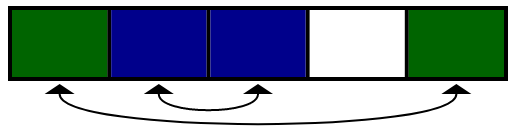
\includegraphics[width=0.4 \columnwidth]{figures/pattern.png}
    \caption{Pattern} 
    \label{fig:pattern} 
\end{figure}

\subsection{Cipher Texts from New Characters}

Sometimes, only moving symbols in not enough to keep information secret. A better why is to substitute symbols with new symbols. These symbols may be letters, numbers or completly new symbols, that are solely invented for the purpose of encrypting information.
In the following exercises the last approach is followed. Again both direction, encryption and decryption, are trained. But this time, instead of having a pattern, there is a symbol table showing how the letters are encrypted. 

\begin{example}
    The cipher text is shown in figure \ref{fig:cipher_number} and the symbol table in figure \ref{fig:symbol_table}. By using the symbol table one can decrypt the cipher text to \code{52}.
\end{example}

\begin{figure} 
    \centering
    
\includegraphics[width=0.2 \columnwidth]{figures/cipher_number.png}
    \caption{Cipher text of an encrypted number} 
    \label{fig:cipher_number} 
\end{figure}

\begin{figure} 
    \centering
    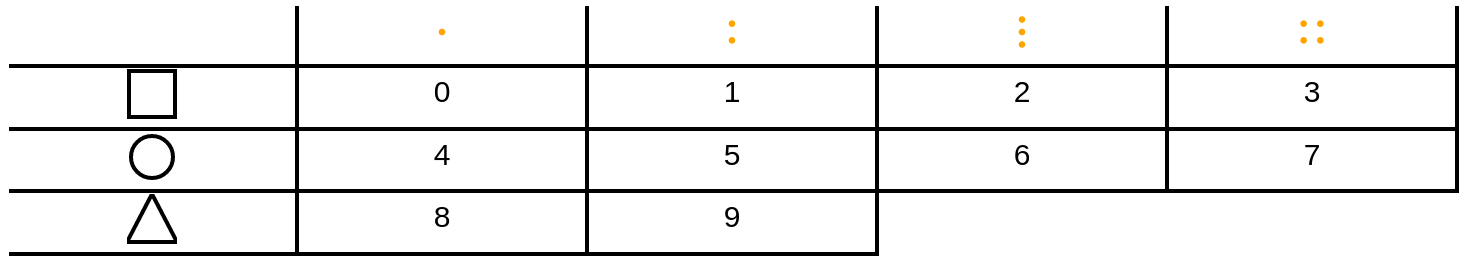
\includegraphics[width=1.0 \columnwidth]{figures/symbol_table.png}
    \caption{Symbol table to encrypt numbers} 
    \label{fig:symbol_table} 
\end{figure}

\section{Learning from Data}

The following exercises are logic-based, combinatorial puzzles. The idea is that pupils need to conclude the solution by a partially completed grid.

\subsection{Row of Trees}

The row of trees is a one dimensional grid i.e a row either of size 3 or 4. In every row there is exactly one tree of every height between 1 and 3 (Fig. \ref{fig:trees_3}) or 4 (Fig. \ref{fig:trees_4}) respectively. At both ends of the row the amount of tree visible from this end of the row is given.
Pupils are given an empty row with only the number of trees seen from both ends of the row and need to place a tree of each height such the aforementioned rules are met.

\begin{figure} 
    \centering
    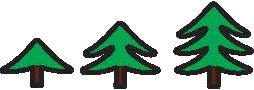
\includegraphics[width=0.4 \columnwidth]{figures/trees_3.png}
    \caption{Trees from height 1 to 3} 
    \label{fig:trees_3} 
\end{figure}

\begin{figure} 
    \centering
    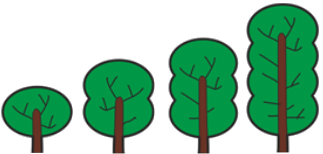
\includegraphics[width=0.4 \columnwidth]{figures/trees_4.png}
    \caption{Trees from height 1 to 4} 
    \label{fig:trees_4} 
\end{figure}

\begin{example}
    For a row of size 3, if given the value 2 for both ends of the row, then one possible solution to the puzzle is shown in figure \ref{fig:tree_row_example}.
\end{example}

\begin{figure} 
    \centering
    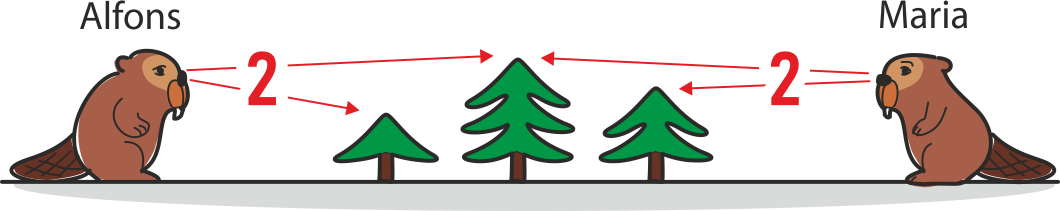
\includegraphics[width=0.8 \columnwidth]{figures/tree_row_example.png}
    \caption{Visualization of the puzzle solution from the tree row example} 
    \label{fig:tree_row_example} 
\end{figure}

\subsection{Tree Sudoku}

Tree sudoku is similar to the well known traditional sudoko with the difference that trees of different heights are placed instead of numbers, and for end of every row and collumn the number of visible trees is given. Otherwise, the puzzle follows the same rules as the row of trees and is either of size 3x3 or 4x4.

\begin{example}
    An example of a 3x3 tree sudoku is shown in figure \ref{fig:tree_sudoku_example}
\end{example}

\begin{figure} 
    \centering
    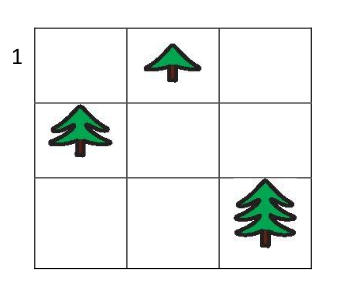
\includegraphics[width=0.4 \columnwidth]{figures/tree_sudoku_example.png}
    \caption{Example of an unsolved 3x3 tree sudoku} 
    \label{fig:tree_sudoku_example} 
\end{figure}
% https://www.bowdoin.edu/~sbarker/teaching/courses/ds/18fall/files/lab4.pdf